\documentclass[10pt,border=4pt]{standalone}
\usepackage{fontspec}
\setmainfont{BeVietnamPro}[Path=D:/IOT_Tools/downloads/fonts/,Extension=.ttf,UprightFont=*-Regular,BoldFont=*-SemiBold]
\usepackage{amsmath}
\usepackage{unicode-math}\setmathfont{Cambria Math}
\usepackage[table]{xcolor}
\usepackage{tikz}
\usetikzlibrary{positioning,arrows.meta,shapes.geometric,calc,fit,backgrounds,decorations.pathreplacing,shadows}
\usepackage{tikz-3dplot}
\usepackage{pgfplots}\pgfplotsset{compat=1.18}
\usepgfplotslibrary{groupplots,fillbetween}
\definecolor{cXanh}{HTML}{1F5A96}\definecolor{cCam}{HTML}{E07B24}\definecolor{cLuc}{HTML}{2E8B57}
\definecolor{cHong}{HTML}{C2397F}\definecolor{cTim}{HTML}{6B4FA0}\definecolor{cXam}{HTML}{5B6770}\definecolor{cVang}{HTML}{D8A51D}
\pgfplotsset{baocao/.style={tick label style={font=\scriptsize}, scaled ticks=false, /pgf/number format/fixed,
  label style={font=\small}, legend style={font=\scriptsize,draw=none,fill=none},
  /pgf/number format/use comma, /pgf/number format/1000 sep={\,}, axis line style={cXam}, major tick style={cXam},
  ymajorgrids, grid style={cXam!20}}}
\pgfplotsset{colormap={baocao}{rgb255=(31,90,150) rgb255=(107,79,160) rgb255=(194,57,127) rgb255=(224,123,36) rgb255=(216,165,29)}}
\pgfkeys{/pgf/number format/assume math mode=true}
\newcommand{\ci}[2]{[#1;\,#2]}\newcommand{\so}[1]{#1}
\begin{document}
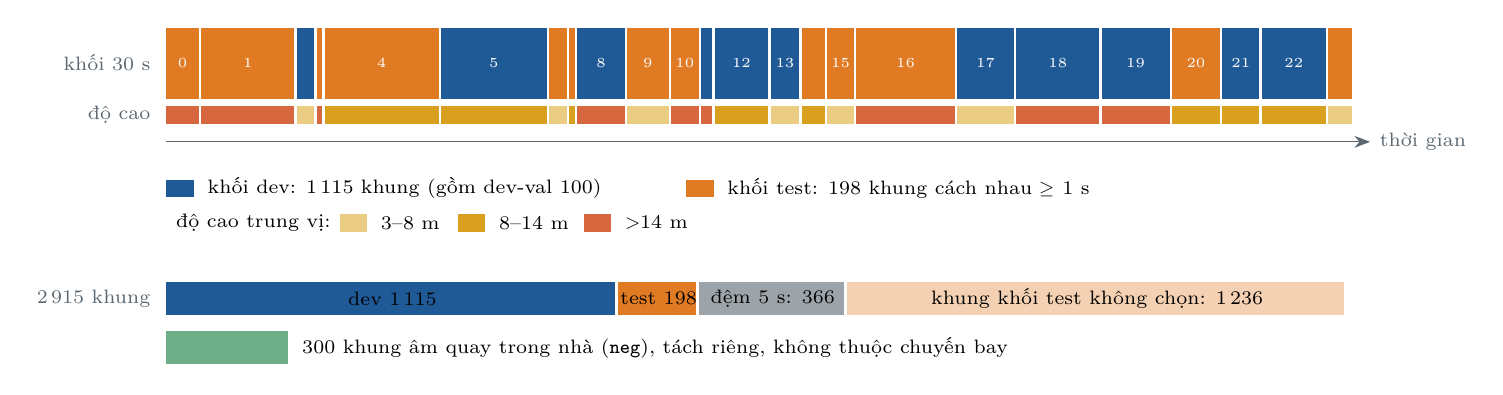
\begin{tikzpicture}[font=\scriptsize, x=1cm, y=1cm]
\fill[cCam] (0.000,0) rectangle ++(0.413,0.9);
\fill[cCam!70!cHong] (0.000,-0.32) rectangle ++(0.413,0.22);
\node[font=\tiny,white] at (0.206,0.45) {0};
\fill[cCam] (0.443,0) rectangle ++(1.179,0.9);
\fill[cCam!70!cHong] (0.443,-0.32) rectangle ++(1.179,0.22);
\node[font=\tiny,white] at (1.032,0.45) {1};
\fill[cXanh] (1.652,0) rectangle ++(0.227,0.9);
\fill[cVang!55] (1.652,-0.32) rectangle ++(0.227,0.22);
\fill[cCam] (1.909,0) rectangle ++(0.070,0.9);
\fill[cCam!70!cHong] (1.909,-0.32) rectangle ++(0.070,0.22);
\fill[cCam] (2.009,0) rectangle ++(1.447,0.9);
\fill[cVang!85!cCam] (2.009,-0.32) rectangle ++(1.447,0.22);
\node[font=\tiny,white] at (2.733,0.45) {4};
\fill[cXanh] (3.486,0) rectangle ++(1.344,0.9);
\fill[cVang!85!cCam] (3.486,-0.32) rectangle ++(1.344,0.22);
\node[font=\tiny,white] at (4.158,0.45) {5};
\fill[cCam] (4.860,0) rectangle ++(0.227,0.9);
\fill[cVang!55] (4.860,-0.32) rectangle ++(0.227,0.22);
\fill[cCam] (5.117,0) rectangle ++(0.070,0.9);
\fill[cVang!85!cCam] (5.117,-0.32) rectangle ++(0.070,0.22);
\fill[cXanh] (5.217,0) rectangle ++(0.603,0.9);
\fill[cCam!70!cHong] (5.217,-0.32) rectangle ++(0.603,0.22);
\node[font=\tiny,white] at (5.519,0.45) {8};
\fill[cCam] (5.850,0) rectangle ++(0.526,0.9);
\fill[cVang!55] (5.850,-0.32) rectangle ++(0.526,0.22);
\node[font=\tiny,white] at (6.113,0.45) {9};
\fill[cCam] (6.406,0) rectangle ++(0.356,0.9);
\fill[cCam!70!cHong] (6.406,-0.32) rectangle ++(0.356,0.22);
\node[font=\tiny,white] at (6.584,0.45) {10};
\fill[cXanh] (6.792,0) rectangle ++(0.140,0.9);
\fill[cCam!70!cHong] (6.792,-0.32) rectangle ++(0.140,0.22);
\fill[cXanh] (6.962,0) rectangle ++(0.680,0.9);
\fill[cVang!85!cCam] (6.962,-0.32) rectangle ++(0.680,0.22);
\node[font=\tiny,white] at (7.302,0.45) {12};
\fill[cXanh] (7.672,0) rectangle ++(0.366,0.9);
\fill[cVang!55] (7.672,-0.32) rectangle ++(0.366,0.22);
\node[font=\tiny,white] at (7.855,0.45) {13};
\fill[cCam] (8.068,0) rectangle ++(0.294,0.9);
\fill[cVang!85!cCam] (8.068,-0.32) rectangle ++(0.294,0.22);
\fill[cCam] (8.392,0) rectangle ++(0.340,0.9);
\fill[cVang!55] (8.392,-0.32) rectangle ++(0.340,0.22);
\node[font=\tiny,white] at (8.562,0.45) {15};
\fill[cCam] (8.763,0) rectangle ++(1.246,0.9);
\fill[cCam!70!cHong] (8.763,-0.32) rectangle ++(1.246,0.22);
\node[font=\tiny,white] at (9.386,0.45) {16};
\fill[cXanh] (10.039,0) rectangle ++(0.726,0.9);
\fill[cVang!55] (10.039,-0.32) rectangle ++(0.726,0.22);
\node[font=\tiny,white] at (10.402,0.45) {17};
\fill[cXanh] (10.795,0) rectangle ++(1.051,0.9);
\fill[cCam!70!cHong] (10.795,-0.32) rectangle ++(1.051,0.22);
\node[font=\tiny,white] at (11.321,0.45) {18};
\fill[cXanh] (11.876,0) rectangle ++(0.865,0.9);
\fill[cCam!70!cHong] (11.876,-0.32) rectangle ++(0.865,0.22);
\node[font=\tiny,white] at (12.308,0.45) {19};
\fill[cCam] (12.771,0) rectangle ++(0.608,0.9);
\fill[cVang!85!cCam] (12.771,-0.32) rectangle ++(0.608,0.22);
\node[font=\tiny,white] at (13.075,0.45) {20};
\fill[cXanh] (13.409,0) rectangle ++(0.469,0.9);
\fill[cVang!85!cCam] (13.409,-0.32) rectangle ++(0.469,0.22);
\node[font=\tiny,white] at (13.644,0.45) {21};
\fill[cXanh] (13.908,0) rectangle ++(0.819,0.9);
\fill[cVang!85!cCam] (13.908,-0.32) rectangle ++(0.819,0.22);
\node[font=\tiny,white] at (14.318,0.45) {22};
\fill[cCam] (14.757,0) rectangle ++(0.299,0.9);
\fill[cVang!55] (14.757,-0.32) rectangle ++(0.299,0.22);
\def\tlW{15.087}

\draw[cXam, -{Stealth[length=2mm]}] (0,-0.55) -- (\tlW+0.2,-0.55) node[right, cXam] {thời gian};
\node[anchor=east, cXam] at (-0.08,0.45) {khối 30 s};
\node[anchor=east, cXam] at (-0.08,-0.21) {độ cao};
% chú giải
\begin{scope}[shift={(0,-1.25)}]
\fill[cXanh] (0,0) rectangle ++(0.35,0.22); \node[anchor=west] at (0.4,0.11) {khối dev: 1\,115 khung (gồm dev-val 100)};
\fill[cCam] (6.6,0) rectangle ++(0.35,0.22); \node[anchor=west] at (7.0,0.11) {khối test: 198 khung cách nhau $\geq$ 1 s};
\node[anchor=west] at (0,-0.33) {độ cao trung vị:};
\fill[cVang!55] (2.2,-0.44) rectangle ++(0.35,0.22); \node[anchor=west] at (2.6,-0.33) {3–8 m};
\fill[cVang!85!cCam] (3.7,-0.44) rectangle ++(0.35,0.22); \node[anchor=west] at (4.1,-0.33) {8–14 m};
\fill[cCam!70!cHong] (5.3,-0.44) rectangle ++(0.35,0.22); \node[anchor=west] at (5.7,-0.33) {$>$14 m};
\end{scope}
% cột tổng
\begin{scope}[shift={(0,-2.75)}]
\foreach \x/\w/\c/\t in {0/5.74/cXanh/{dev 1\,115},5.74/1.02/cCam/{test 198},6.76/1.88/cXam!60/{đệm 5 s: 366},8.64/6.36/cCam!35/{khung khối test không chọn: 1\,236}}
  {\fill[\c] (\x,0) rectangle ++(\w-0.04,0.42); \node[font=\scriptsize] at (\x+\w/2,0.21) {\t};}
\node[anchor=east, cXam] at (-0.08,0.21) {2\,915 khung};
\fill[cLuc!70] (0,-0.62) rectangle ++(1.54,0.42); \node[anchor=west] at (1.6,-0.41) {300 khung âm quay trong nhà (\texttt{neg}), tách riêng, không thuộc chuyến bay};
\end{scope}
\end{tikzpicture}

\end{document}
